\begin{ZhChapter}

    \chapter{Methodology}
    In this section, we will introduce the Structured Semantics and Generation Embedded Network Intrusion Detection System (S2GE-NIDS) architecture and detail its operational workflow, clearly delineating each step from preprocess module through embedding module and Mahalanobis distance anomaly processes.
    \section{Architecture} %Chapter 3.1
    The architecture of S2GE-NIDS is presented as Figure \ref{fig:Architecture}. The further description will begin in the section 3.1.1.

    \begin{figure*}[htbp]
        \centering
        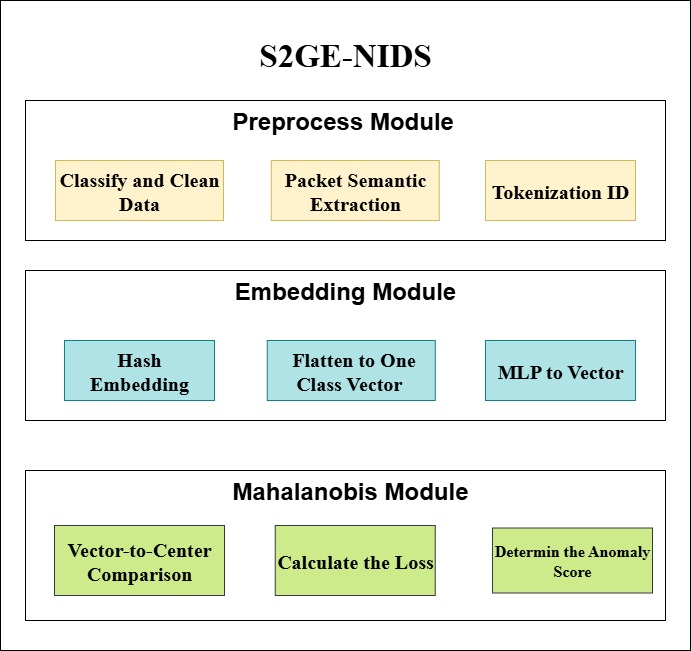
\includegraphics[width = 0.8\textwidth]{image/architecture.png}
        \caption{Architecture of S2GE-NIDS}
        \label{fig:Architecture}
    \end{figure*}



    \subsection{Preprocess Module}
    In the preprocessing phase, as shown in Figure~\ref{fig:preprocessModule}, we will perform the following steps: data file classification and cleaning, packet semantic extraction, and tokenization. These steps are designed to transform raw network traffic into structured representations suitable for semantic embedding and anomaly detection.


    \begin{figure*}[htbp]
        \centering
        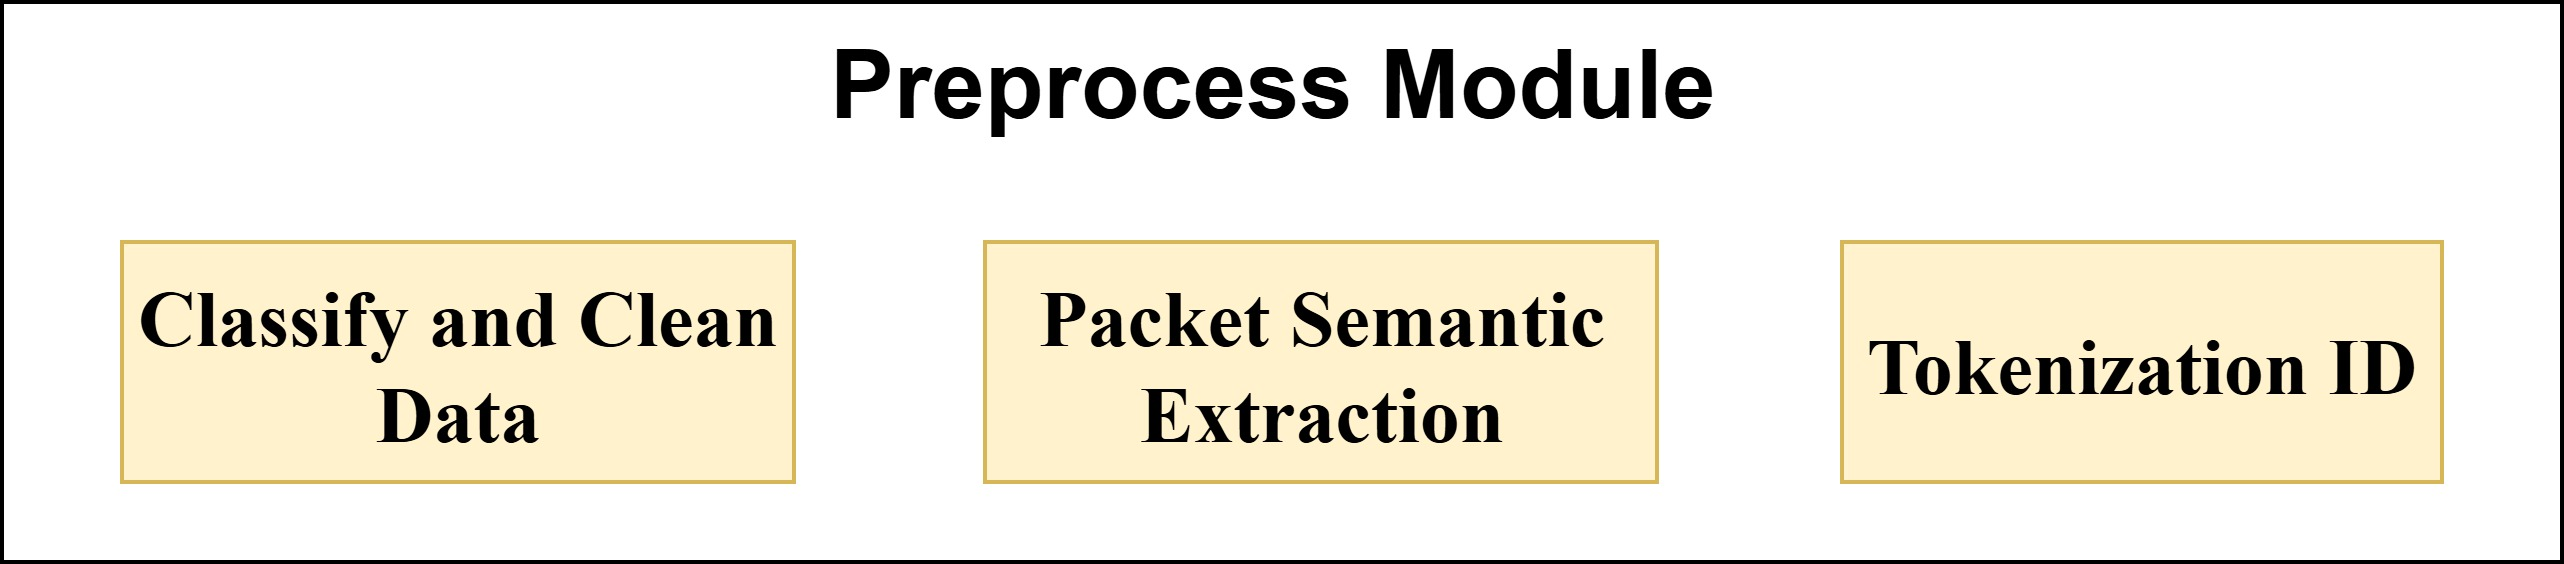
\includegraphics[width = 0.8\textwidth]{image/preprocessModule.png}
        \caption{Architecture of Preprocess Module }
        \label{fig:preprocessModule}
    \end{figure*}


    \subsubsection{Classify and Clean Data}
    In S2GE, the dataset is partitioned into three distinct subsets to facilitate effective model training and evaluation: 70\% of the data is allocated for training, 15\% for validation, and the remaining 15\% for testing.
    \begin{figure*}[htbp]
        \centering
        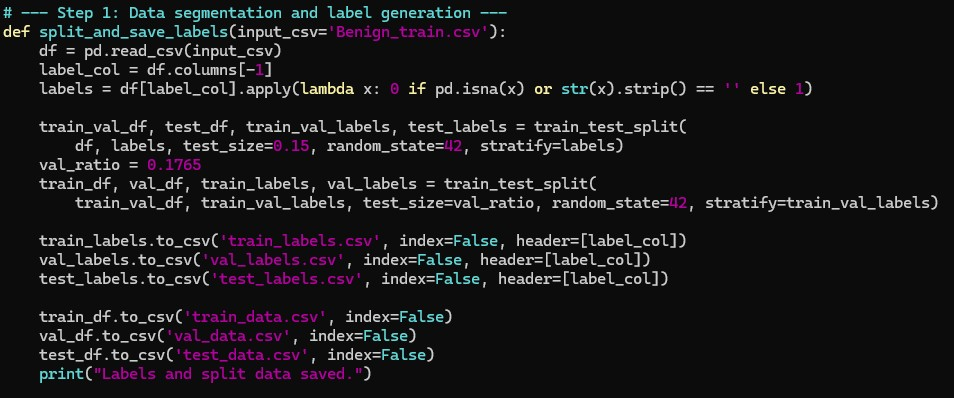
\includegraphics[width = 0.8\textwidth]{image/datasplit.jpg}
        \caption{Data split process}
        \label{fig:preprocessModule}
    \end{figure*}

    The first step in the preprocessing pipeline involves selecting and filtering data files to ensure their suitability for subsequent analysis. In this study, network traffic is collected and stored in the Comma-Separated Values (CSV) format, a widely adopted and flexible tabular data structure. CSV files are particularly well-suited for structured data representation due to their ease of parsing, compact storage, and seamless integration with mainstream data analysis libraries such as pandas, and NumPy in Python.

    After selecting the data format, the raw data are merged into a unified DataFrame and subjected to a series of cleaning procedures. First, all column names are normalized by removing extraneous whitespace and standardizing naming conventions where necessary to ensure consistency across feature dimensions. Next, rows containing missing or undefined entries are removed to prevent bias in downstream training. Finally, columns consisting solely of zeros are discarded.

    During this stage, the resulting dataset serves as the foundation for the subsequent tokenization and embedding stages.

    \subsubsection{Packet Semantic Extraction}

    Packet semantic extraction refers to the process of identifying and transforming raw packet-level attributes into semantically meaningful representations that facilitate accurate anomaly detection. As summarized in Table~2.1, a set of representative features such as \textit{Destination Port}, \textit{Protocol Type}, \textit{Flow Duration}, \textit{Packet Length}, \textit{Flow Bytes per Second}, \textit{TCP Flag Counts}, and \textit{Connection Count} have been consistently validated in prior studies as effective indicators of anomalous or malicious traffic behavior.





    \subsubsection{Tokenization ID}
    Following the feature extraction phase, the structured network traffic attributes undergo a tokenization process, where in categorical feature fields are transformed into discrete, semantically interpretable string tokens. These tokens form the foundation for subsequent vector embedding. The dataset comprises multiple structured records, each containing various categorical attributes such as \texttt{Destination Port}, \texttt{Protocol Type}, and \texttt{Source IP Address} that capture the behavioral characteristics of individual traffic flows. By converting these symbolic fields into tokenized string representations, the module preserves both the identity and contextual meaning of traffic patterns, thereby enabling more effective semantic encoding in later stages.



    Table~\ref{tab:token_example} shows the tokenization method employed, where each feature is transformed by concatenating its field name and corresponding value with a colon separator to form a token. For example, the field name "DestinationPort" combined with the value "80" becomes the token "DestinationPort:80"; similarly, "FlowDuration" with "0.32817" becomes "FlowDuration:0.32817", and "ProtocolType" with "TCP" becomes "ProtocolType:TCP".

    \begin{table*}[htbp]
        \centering
        \caption{Example of Tokenization Process}
        \label{tab:token_example}
        \vspace{1em}
        \makebox[\linewidth][c]{
            \renewcommand\arraystretch{1.2}{
                \begin{tabular}{| l | l | l |}
                    \hline
                    \textbf{Field Name} & \textbf{Field Value} & \textbf{Token}       \\
                    \hline
                    Destination Port    & 80                   & DestinationPort:80   \\
                    Flow Duration       & 0.32817              & FlowDuration:0.32817 \\
                    Protocol Type       & TCP                  & ProtocolType:TCP     \\
                    \hline
                \end{tabular}
            }}
    \end{table*}



    \subsection{Embedding Module} %3.1.2
    To convert network packet features into vector representations that can be processed by the module, this architecture employs an efficient embedding module. Figure~\ref{fig:EmbeddedModule} shows the entire process includes hash embedding, flatten to a one-class vector, and using a multi-layer perceptron (MLP) to vector.

    \begin{figure*}[htbp]
        \centering
        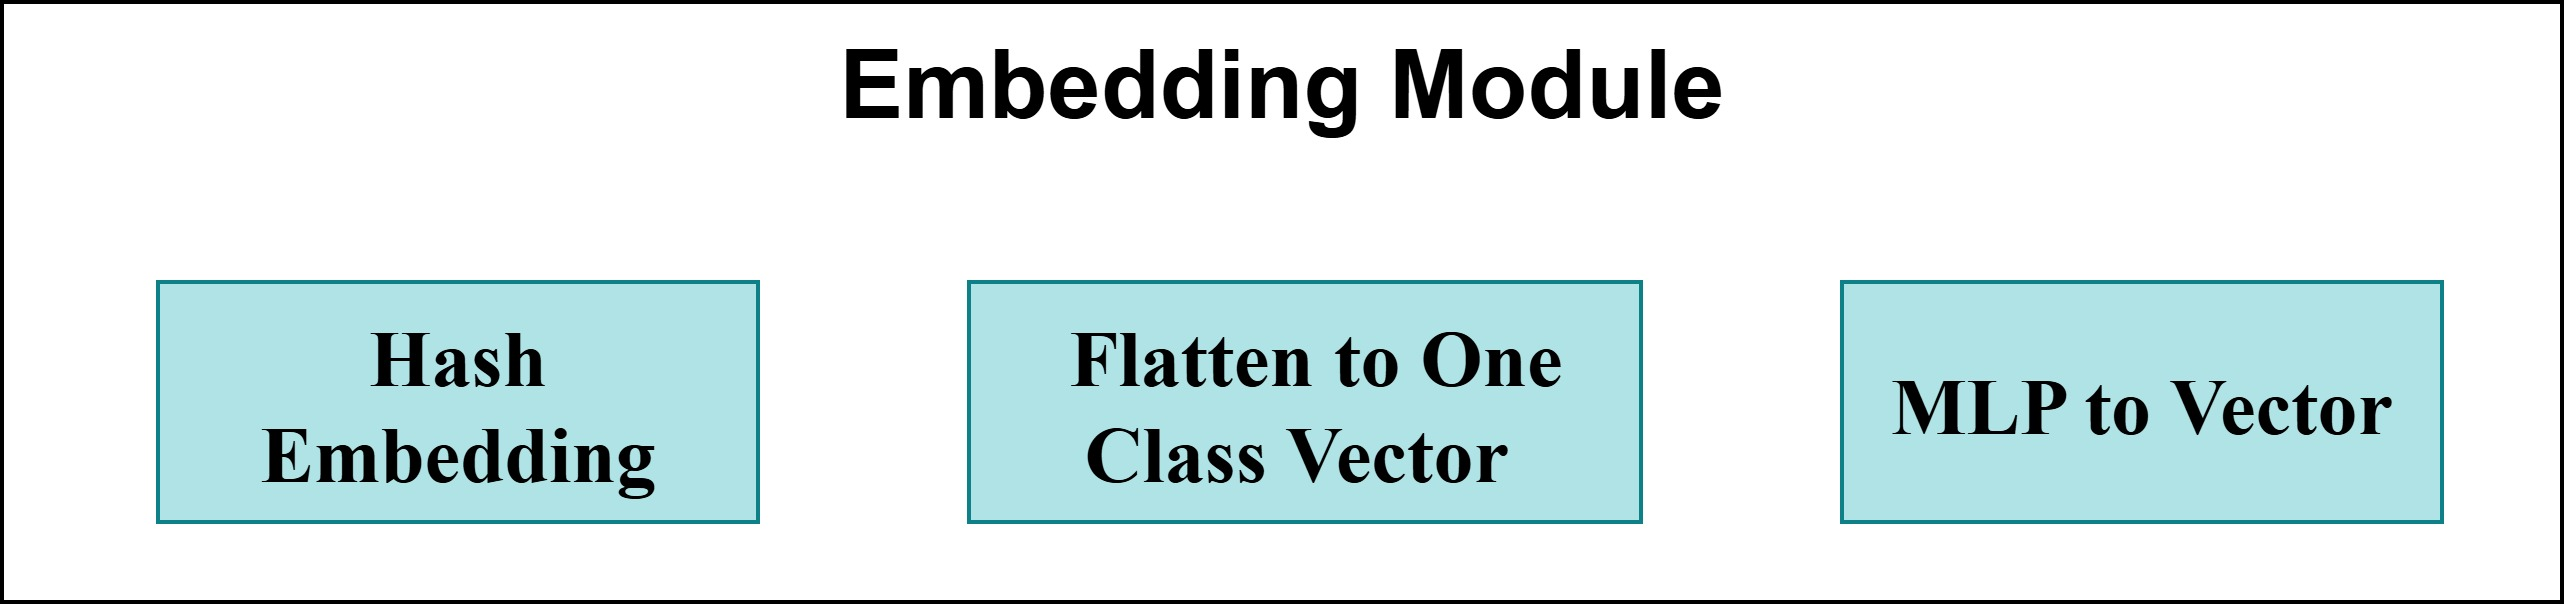
\includegraphics[width = 0.8\textwidth]{image/EmbeddingModule.jpg}
        \caption{Architecture of Preprocess Module }
        \label{fig:EmbeddedModule}
    \end{figure*}

    \subsubsection{Hash Embedding} %3.1.2.1
    Hash embedding~\cite{li2024embedding} is a lightweight vectorization technique that utilizes non-cryptographic hashing to encode tokenized field-value pairs into fixed-size, trainable embeddings. In this study, we adopt the MurmurHash3 algorithm, an efficient and widely used hash function, to map each token to a specific position in the embedding table. Its advantages include fast computation, uniform distribution, and language-independent implementation, making it well-suited for scalable anomaly detection in IoT environments.

    In this study, the embedding table is theoretically designed as a fixed-size matrix of dimension \(223 \times 223\), where each cell contains an 8-dimensional embedding vector representing tokens hashed via the MurmurHash3 function and mapped through modulo operation. This fixed-size matrix structure facilitates uniform feature distribution and ensures a consistent input dimension for downstream machine learning models.

    In the design of the hash embedding table, the choice of the table size plays a critical role in the efficiency and effectiveness of the hashing process. We select the table size as a prime number, specifically 223, resulting in an embedding table of size $223 \times 223 = 49,729$.

    According to Theorem 11.9~\cite{cormen2022introduction}, when storing $n$ keys in a hash table of size $m = n^2$ using a hash function $h$ randomly selected from a universal class of hash functions, the probability of any collisions is less than $\frac{1}{2}$. Moreover, it is well established in the literature that choosing a prime number as the hash table size reduces the likelihood of collisions and promotes a uniform distribution of hash values across the table.

    Considering the practical memory constraints typical in Internet of Things (IoT) devices many of which feature memory capacities around 256 KB or multiples thereof the selection of a prime number close to 256, such as 223, represents a strategic balance between memory efficiency and hashing performance. This design choice facilitates efficient deployment in resource-constrained IoT environments without incurring excessive memory overhead.

    \begin{figure*}[htbp]
        \centering
        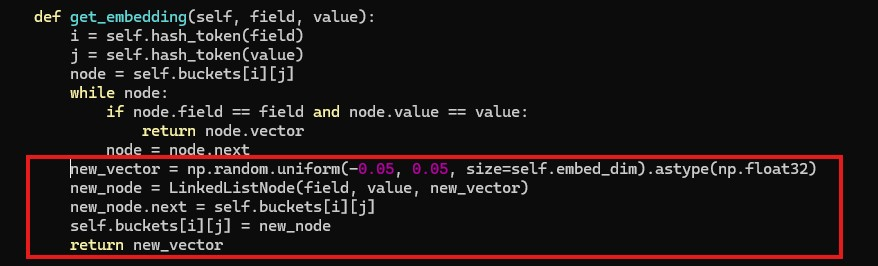
\includegraphics[width = 0.8\textwidth]{image/initial.jpg}
        \caption{Initial the Embedding Table}
        \label{fig:Initial}
    \end{figure*}


    However, due to the inevitability of hash collisions where multiple distinct tokens map to the same index using a static three-dimensional matrix can lead to vector overwriting and information loss. To address this, the embedding table is implemented in practice as a dynamic linked list structure using a dictionary-based approach. This implementation allows flexible storage of multiple embedding vectors corresponding to collided tokens at the same index, thus preserving embedding integrity and optimizing memory usage.

    During the output stage, the embedding vectors corresponding to all tokens within a single data row are flattened into a one-dimensional vector, which serves as input to subsequent models such as MLP. Although this practical implementation differs from the theoretical fixed three-dimensional matrix, the overall architecture and core objectives remain consistent, aiming to provide an efficient and representative semantic vector encoding.

    This divergence between theory and implementation reflects a trade-off between resource constraints and collision handling. The dynamic linked list structure offers scalability and ease of maintenance, enhancing both the usability and computational efficiency of the embedding table while ensuring the completeness of the vector representations.


    To determine the target index for each token, each vector is initialized randomly and refined during module training as in Figure~\ref{fig:Initial}.

    From the above example, as shown in Figure~\ref{fig:hashembedding}, the field name \texttt{Destination\_Port} yields an index of 129, while its value \texttt{80} maps to 166; these indices are used to locate specific embedding vectors.

    \begin{figure*}[!t]
        \centering
        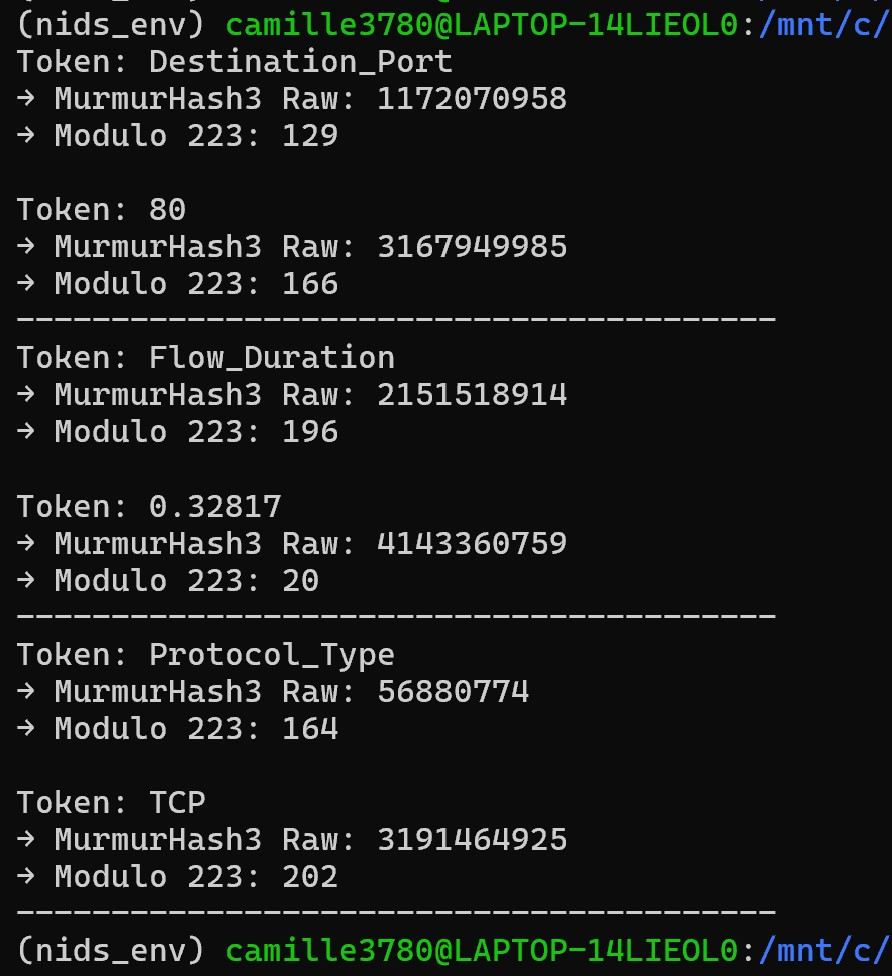
\includegraphics[width = 0.4\textwidth]{image/2025-06-30 002218.jpg}
        \caption{Hash Embedding Process}
        \label{fig:hashembedding}
    \end{figure*}


    \begin{figure*}[htbp]
        \centering
        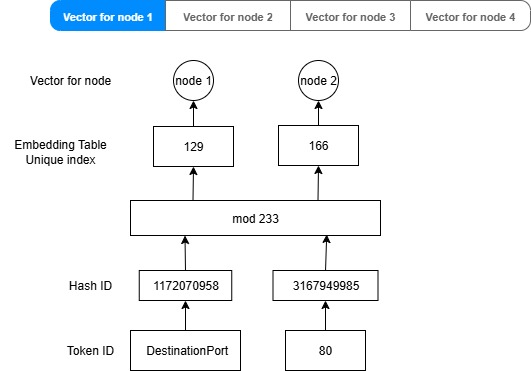
\includegraphics[width = 0.5\textwidth]{image/EmbeddingFlow.jpg}
        \caption{Double Hashing with Linked List for Embedding Storage}
        \label{fig:HashEmbeddingFlow}
    \end{figure*}


    The process begins with a \textit{Token ID} shown as Figure~\ref{fig:HashEmbeddingFlow}, such as the categorical feature \texttt{DestinationPort} and its corresponding value 80. This Token ID is first processed through a hash function \textcircled{1} to generate a large integer hash value (e.g., 3167949985). This step effectively converts high-dimensional sparse features into uniformly distributed integers, reducing feature sparsity and enabling efficient indexing. Formally:
    \begin{equation}
        \text{Hash ID} = \text{Hash}(\text{Token ID})
    \end{equation}

    To map this hash value into the embedding table, a modulo operation is applied using the table size \( m \) \textcircled{2} (here, \( m = 223 \)) yielding a unique index \textcircled{3} within the embedding table (e.g., 166). This index corresponds to a primary slot in the embedding table.

    Due to the possibility of hash collisions where multiple distinct tokens may hash to the same modulo index a \textit{dynamic linked list} \textcircled{4} is employed to handle such conflicts. When a collision occurs, additional embedding vectors are stored in linked nodes associated with the initial index.

    In this process, each embedding vector is identified by its unique index after modulo operation (e.g., 129 for another hash value). The system checks the embedding table entry at this index:

    \begin{itemize}
        \item If the table is free or matches the token, the embedding vector is stored or retrieved directly.
        \item If the table is occupied by a collision, a pointer will link to the next node in the list.
    \end{itemize}


    \begin{figure*}[htbp]
        \centering
        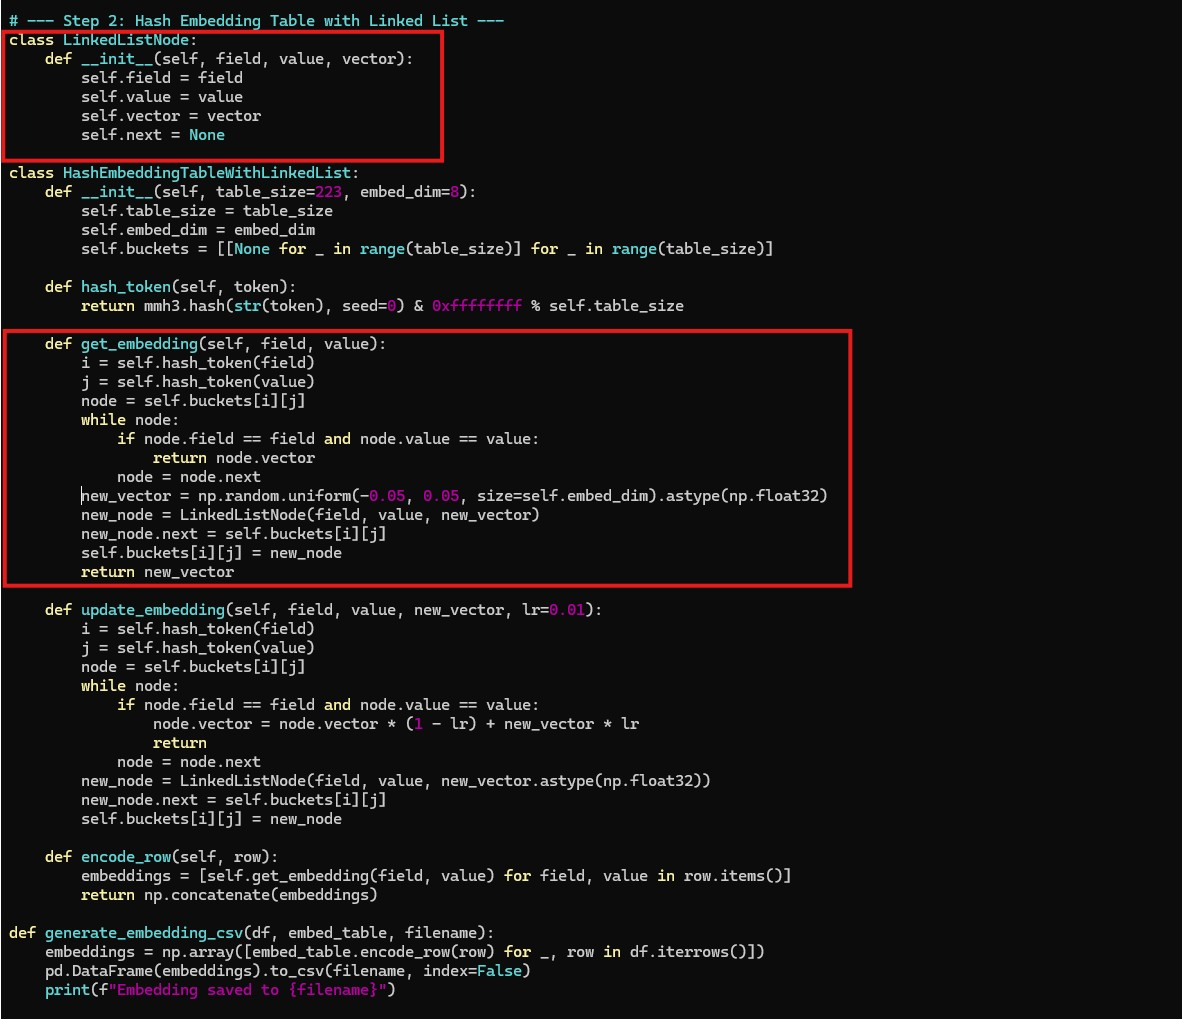
\includegraphics[width = 0.8\textwidth]{image/LinklistCode.jpg}
        \caption{Dynamic Linked List of Embedding Table}
        \label{fig:link}
    \end{figure*}

    As shown in Figure~\ref{fig:link}, this illustrates the double hashing technique combined with a dynamic linked list structure to efficiently store embedding vectors in a fixed-size embedding table.







    \subsubsection{Flatten to One Class Vector}
    The flatten operation concatenates the tokenized embeddings from each column into a single vector for input to the next stage of the pipeline. Table~\ref{tab:token_embedding_table} shows example embedding vectors for individual tokens.


    \begin{table}[htbp]
        \scriptsize
        \centering
        \renewcommand{\arraystretch}{1.2}
        \caption{Hash Values in the Embedding Table}
        \vspace{1em}
        \begin{tabular}{| c | c | c | l |}
            \hline
            \textbf{Token}    & \textbf{Hash} & \textbf{Mod=223} & \textbf{Embedding Vector}                                                        \\
            \hline
            Destination\_Port & 1172070958    & 129              & [0.091251, 0.332761, 0.725833, 0.472719, 0.937337, 0.429821, 0.046714, 0.055904] \\
            80                & 3167949985    & 166              &                                                                                  \\
            \hline
            Flow\_Duration    & 2151518914    & 196              & [0.012133, 0.628566, 0.035354, 0.851932, 0.437327, 0.968118, 0.040445, 0.434074] \\
            0.32817           & 4143360759    & 20               &                                                                                  \\
            \hline
            Protocol\_Type    & 56880774      & 164              & [0.044425, 0.674622, 0.362488, 0.078440, 0.640184, 0.862753, 0.158649, 0.322290] \\
            TCP               & 3191464925    & 202              &                                                                                  \\
            \hline
        \end{tabular}
        \label{tab:token_embedding_table}
    \end{table}



    \begin{figure}[htbp]
        \centering
        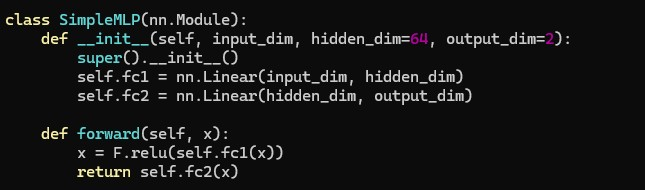
\includegraphics[width = 0.8\textwidth]{image/flattern.jpg}
        \caption{Process of Flattern to One Class Vector}
        \label{fig:FF}
    \end{figure}

    Figure ~\ref{fig:FF} shows the each feature-value pair in the row, its embedding vector is obtained and appended to a list.


    \begin{figure}[htbp]
        \centering
        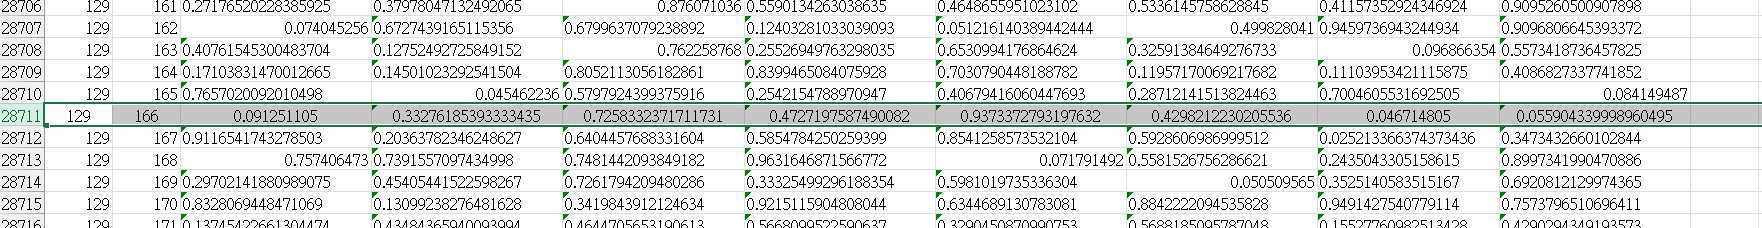
\includegraphics[width = 1\textwidth]{image/129_166.jpg}
        \caption{Example for DestinationPort:80 [129,166]}
        \label{fig:vector}
    \end{figure}
    \begin{figure}[htbp]
        \centering
        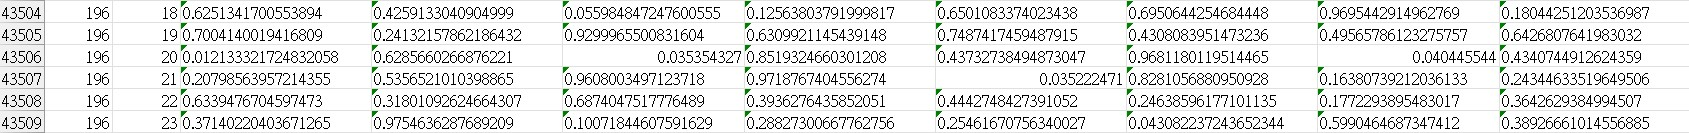
\includegraphics[width = 1\textwidth]{image/196_20.jpg}
        \caption{Example for FlowDuration:0.32817 [196,20]}
        \label{fig:vector}
    \end{figure}

    \begin{figure}[htbp]
        \centering
        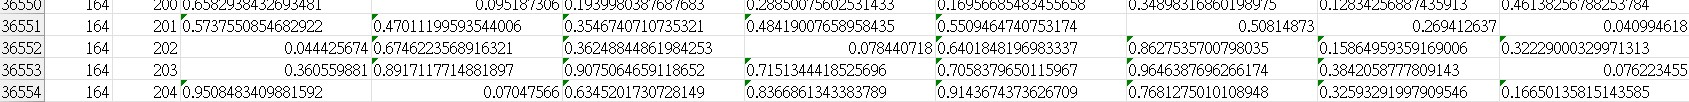
\includegraphics[width = 1\textwidth]{image/164_202.jpg}
        \caption{Example for ProtocolType:TCP [164,202]}
        \label{fig:vector}
    \end{figure}

    % \newpage
    Each row corresponds to a flattened embedding vector generated by concatenating hashed representations of multiple feature fields. The numerical values, ranging between 0 and 1, represent the individual dimensions of the embedding vectors, which have undergone normalization or activation transformations.

    \begin{figure}[htbp]
        \centering
        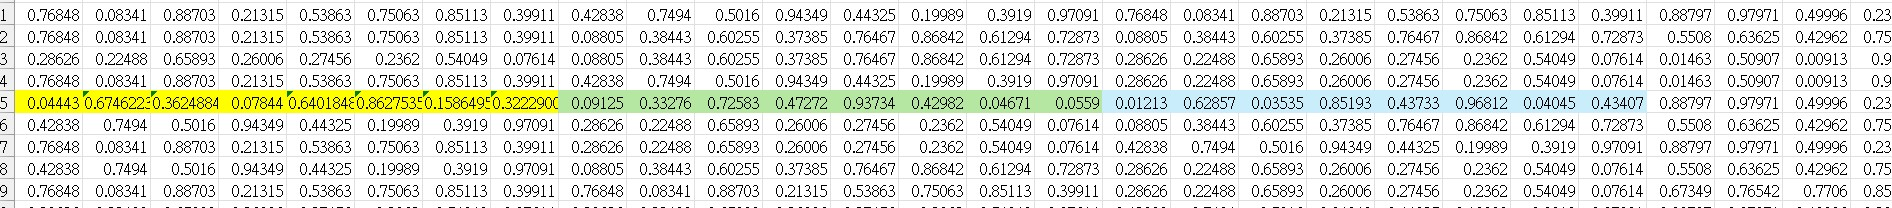
\includegraphics[width = 1\textwidth]{image/merge.jpg}
        \caption{Example rows of Flattened Embedding Vectors}
        \label{fig:merge}
    \end{figure}


    Figure~\ref{fig:merge} shows the packet vectors after flattening, where the highlighted rows (indices 129 and 166) exemplify samples with distinctive embedding patterns across multiple dimensions.





    These embedding vectors serve as foundational inputs to deeper models, such as MLPs~\cite{taud2017multilayer}, facilitating the extraction of higher-level semantic features and improving detection accuracy.

    \subsubsection{MLP to Vector}
    To integrate the multiple field semantic vectors extracted from the embedding table for each packet into a unified semantic representation, a MLP encoder module is introduced. The main task of this module is to map a flattened one-dimensional vector \(\mathbf{x} \in \mathbb{R}^{F \times d}\) to a fixed-dimensional semantic feature vector \(\mathbf{z} \in \mathbb{R}^k\), where \(F\) is the number of fields, \(d\) is the embedding dimension of each field, and \(k\) is the dimension of the output vector.



    The MLP is composed of multiple fully connected layers as shown in Figure~\ref{fig:mlp}.
    \begin{figure}[htbp]
        \centering
        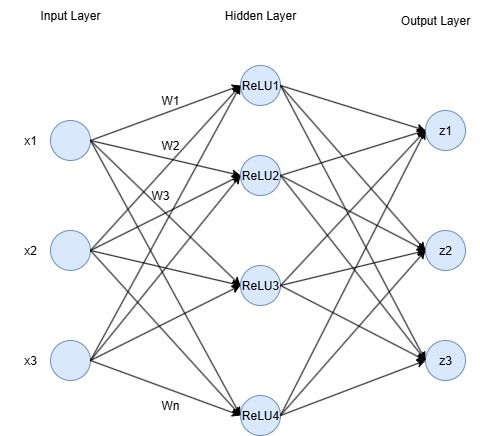
\includegraphics[width = 0.4\textwidth]{image/MLP.jpg}
        \caption{Multiple fully connected layers of the MLP}
        \label{fig:mlp}
    \end{figure}


    \begin{figure}[htbp]
        \centering
        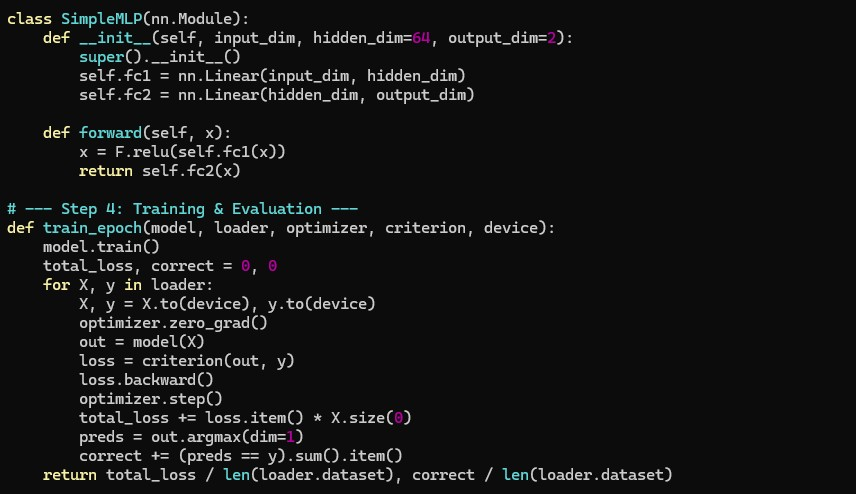
\includegraphics[width = 0.7\textwidth]{image/MLP_code.jpg}
        \caption{MLP Module}
        \label{fig:MLP_code}
    \end{figure}

    Figure~\ref{fig:MLP_code} shows the multi-layer perceptron (MLP) encoder employed in our system. It is designed to transform the concatenated embedding vectors into a fixed-length semantic feature vector. The implemented MLP consists of three fully connected layers with intermediate batch normalization, Rectified Linear Unit(ReLU) activation, and dropout regularization to improve generalization and prevent overfitting~\cite{ioffe2015batch}.

    Specifically, the first layer maps the input vector of dimension \texttt{input\_dim} to a 128-dimensional hidden representation, followed by batch normalization and ReLU activation. A dropout layer with a dropout rate of 0.4 is applied to reduce overfitting. The second layer further reduces the representation from 128 to 64 dimensions, followed again by batch normalization, ReLU, and dropout. Finally, the third layer projects the 64-dimensional vector to the desired embedding dimension (default 16), producing the compact semantic embedding output.

    The forward pass of the MLP applies this sequential transformation to the input feature vector, generating the output embedding used for downstream tasks.

    For training, the MLP model is optimized using the Adam optimizer~\cite{zhang2018improved} with a learning rate of $5 \times 10^{-4}$ and weight decay of $1 \times 10^{-3}$. The mean squared error (MSE)~\cite{garcia2024review} loss is adopted as the training criterion. The training loop iterates over the dataset for 30 epochs, processing data in batches provided by a PyTorch DataLoader wrapping a custom dataset class that converts input data into float tensors.

    Batch normalization and dropout applied in each hidden layer enhance model robustness, while the optimizer parameters facilitate effective convergence during training.

    \begin{figure}[htbp]
        \centering
        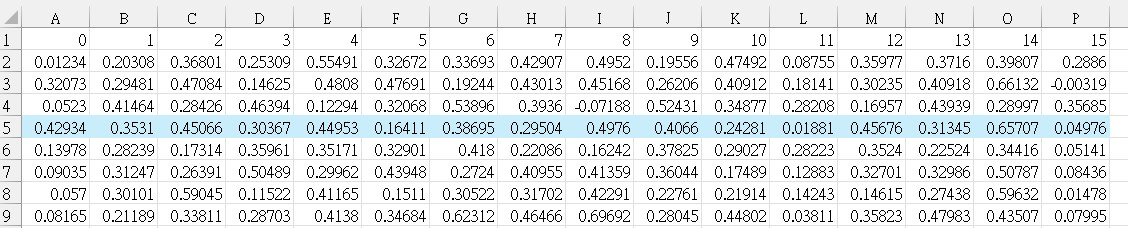
\includegraphics[width = 0.9\textwidth]{image/mlp_result.jpg}
        \caption{Semantic Vector Output}
        \label{fig:MLP_rs}
    \end{figure}
    As presented in Figure~\ref{fig:MLP_rs}, the Mahalanobis distances computed from the semantic embeddings is presented. Each row corresponds to a sample index and its respective Mahalanobis distance value. These distances quantitatively represent how far each sample deviates from the learned mean distribution in the embedding space, serving as an indicator of potential anomalies. Higher distance values suggest greater deviation and a higher likelihood of being anomalous.

    %the full connection and ReLU activation from input layer to hidden layer to output layer
    \subsection{Mahalanobis Distance Module}%3.1.3.1
    In the final stage of the S2GE-NIDS framework, Mahalanobis Distance is applied to evaluate whether a semantic vector deviates significantly from the expected distribution of normal traffic. This metric is particularly effective for high-dimensional anomaly detection, as it accounts for feature correlations and variance.

    \begin{figure*}[htbp]
        \centering
        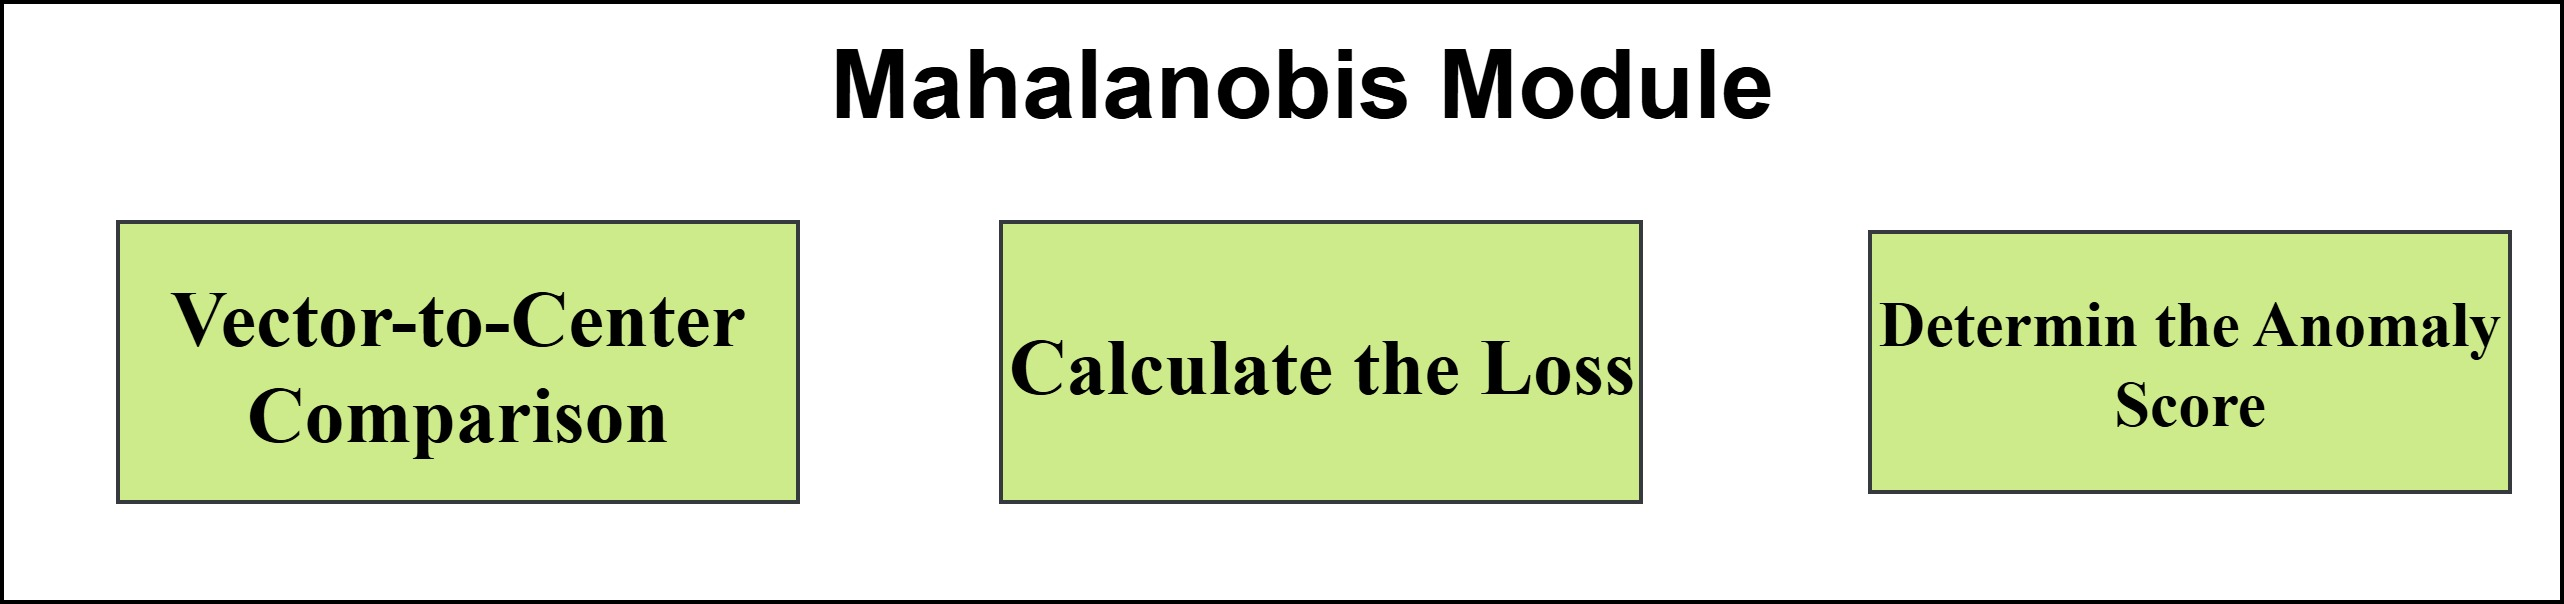
\includegraphics[width = 0.8\textwidth]{image/MahalanobisModule.jpg}
        \caption{Architecture of Preprocess Module }
        \label{fig:MahalanobisModule}
    \end{figure*}


    \begin{figure*}[htbp]
        \centering
        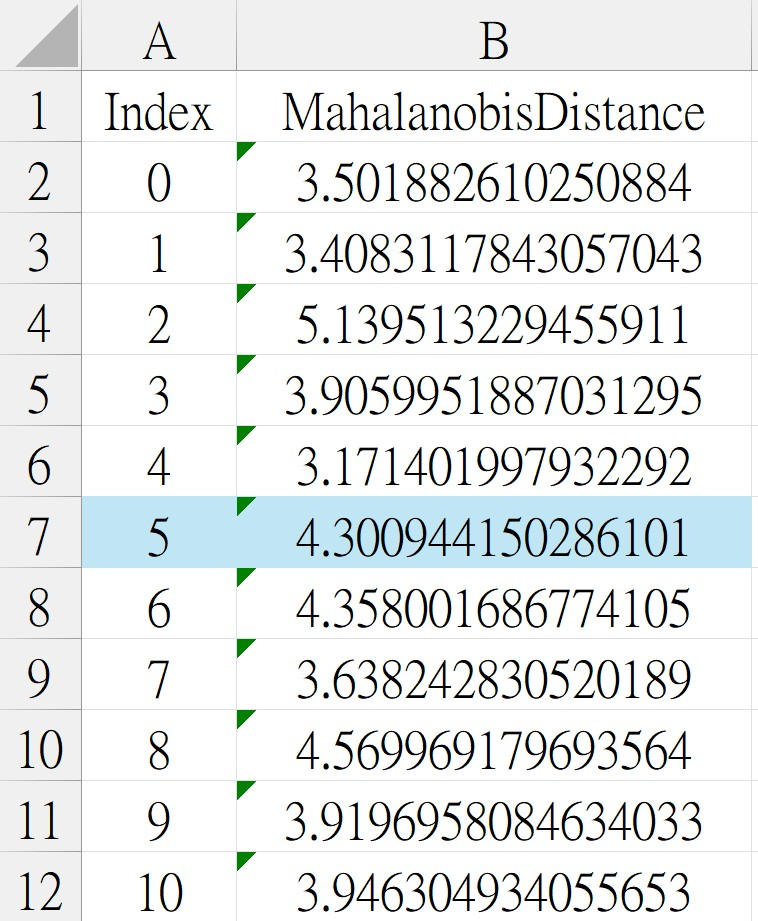
\includegraphics[width = 0.4\textwidth]{image/mh_rs.jpg}
        \caption{Mahalanobis Distances of Result}
        \label{fig:mh_rs}
    \end{figure*}



    \subsubsection{Vector-to-Center Comparison}
    To enhance anomaly detection, S2GE-NIDS incorporates a center loss mechanism. During training, all semantic vectors corresponding to ``normal'' samples are aggregated to compute a center point \(c\).



    By accounting for the variability and correlation of each feature, the module is able to more accurately detect abnormal samples that are ``off-center.''

    During the training process, the Mahalanobis distance calculation for each data point first uses the Euclidean distance to estimate the mean of the latent space. In addition, the variance of each latent dimension is also calculated to facilitate the calculation and optimization of the loss function in the subsequent stage.


    \begin{equation}
        D_M(z) = \sqrt{(z - c)^T \Sigma^{-1} (z - c)}
        \label{eq:mahalanobiseq}
    \end{equation}

    $z$ is the semantic vector of the input sample, $c$ is the center vector of normal samples, and $\Sigma^{-1}$ is the inverse of the covariance matrix of the training data's embedding vectors.

    Because the Mahalanobis distance at this stage needs to be calculated using the covariance matrix. If the covariance matrix is not positive definite, the inverse matrix calculation will be wrong, resulting in abnormal distance values that may appear negative~\cite{tolstikhin2021mlp}.

    \text{The eigenvalues of the covariance matrix are:}
    \[
        \boldsymbol{\lambda} =
        \begin{bmatrix}
            0.01926464, & 0.00316234, & 0.00188263, & 0.00011551, \\
            0.00022377, & 0.00049849, & 0.00072437, & 0.00062288
        \end{bmatrix}
    \]



    \begin{figure*}[htbp]
        \centering
        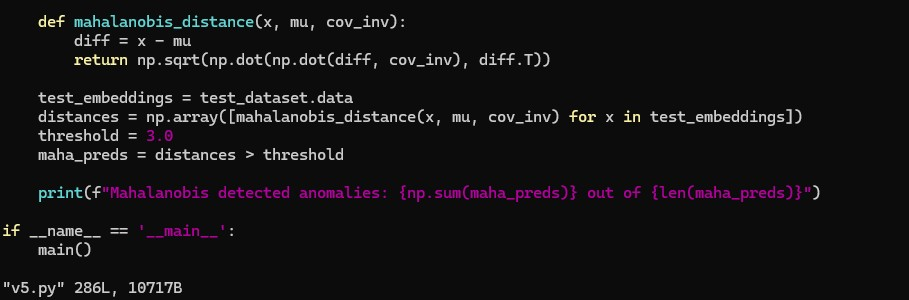
\includegraphics[width = 0.7\textwidth]{image/3131.jpg}
        \caption{Mahalanobis Distance Process}
        \label{fig:3131}
    \end{figure*}

    Fig~\ref{fig:3131} shows the Mahalanobis during the training process, calculate for each data point first uses the Euclidean distance to estimate the mean of the latent space. In addition, the variance of each latent dimension is also calculated to facilitate the calculation and optimization of the loss function in the subsequent stage.


    \begin{figure*}[htbp]
        \centering
        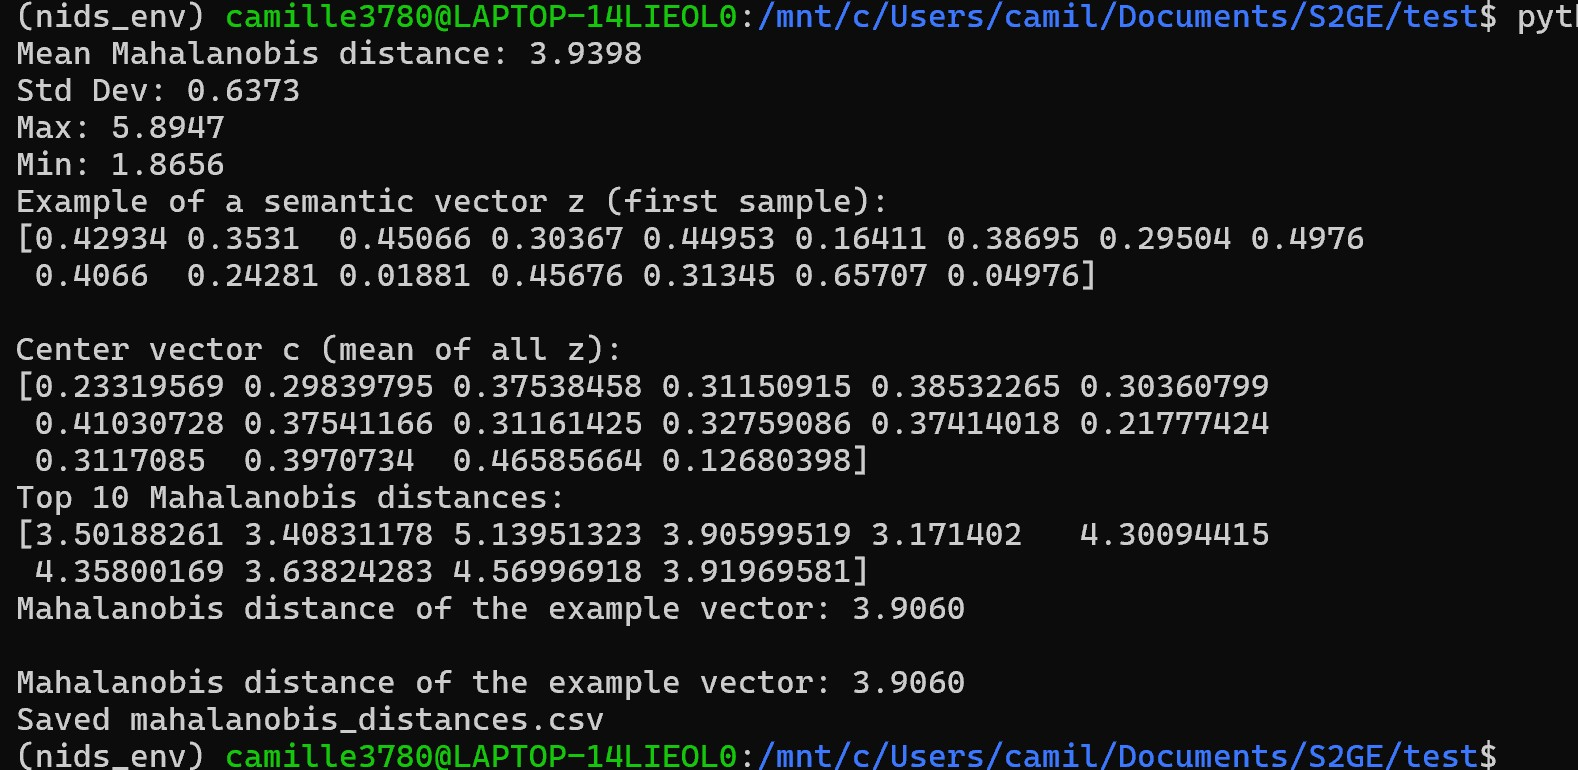
\includegraphics[width = 0.7\textwidth]{image/mean.jpg}
        \caption{Mahalanobis Distance Statistics Data}
        \label{fig:mean}
    \end{figure*}

    As presented in Figure~\ref{fig:mean}, shows a portion of the flattened semantic embedding vectors produced by the MLP encoder. Each highlighted row corresponds to a sample's embedding vector in the 16-dimensional semantic space. These vectors are the transformed representations of the original features, capturing underlying semantic information relevant for anomaly detection. The values across the dimensions reflect complex learned features, which the Mahalanobis distance leverages to assess anomaly scores effectively.


    \subsubsection{Calculate the Loss} %3.1.3.2
    Figure~\ref{fig:3132} shows the training loss progression of the MLP model over 10 epochs. The loss is computed using the MSE between the predicted outputs and the first 16 dimensions of the input embedding vectors, reflecting the model's ability to reconstruct or approximate the latent representations. During each epoch, the model parameters are optimized via backpropagation with the Adam optimizer, and the average loss per epoch is reported. The steadily decreasing loss curve indicates effective convergence and improved model fitting over the training process.
    \begin{figure*}[htbp]
        \centering
        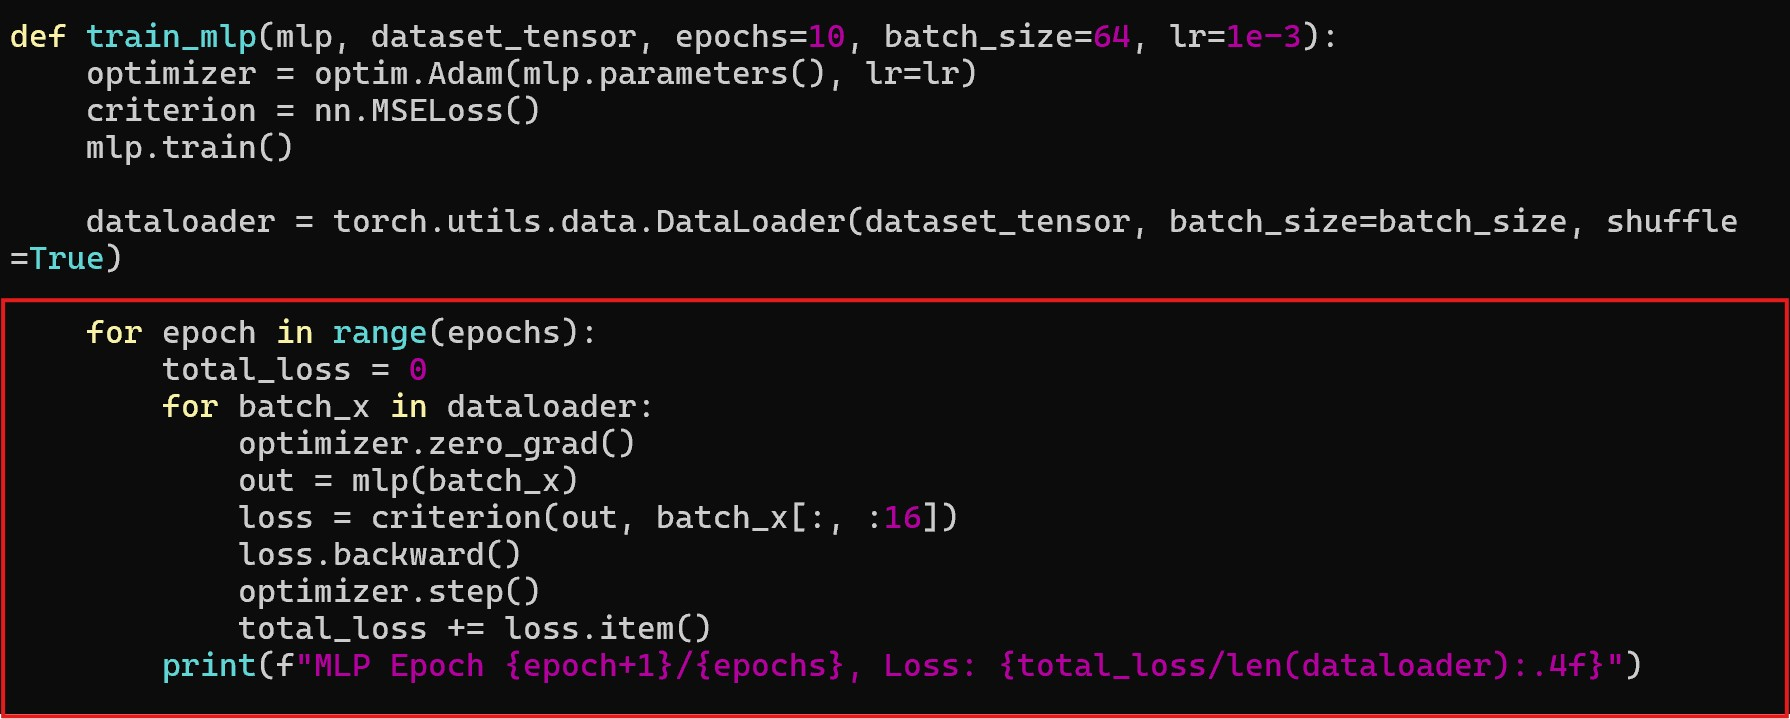
\includegraphics[width = 0.7\textwidth]{image/Loss.jpg}
        \caption{The Loss of MLP Training process}
        \label{fig:3132}
    \end{figure*}


    \begin{itemize}
        \item The loss is defined as:
    \end{itemize}

    \begin{equation}
        \mathcal{L} = \frac{1}{N} \sum_{i=1}^{N} \| z_i - c \|^2
        = \frac{1}{N} \sum_{i=1}^{N} \sum_{j=1}^{d} (z_{ij} - c_j)^2
        \label{eq:centerloss}
    \end{equation}

    $z_i \in \mathbb{R}^d$ is the embedding vector obtained after the $i$th input passes through the Semantic Encoder,
    $c \in \mathbb{R}^d$ is the center point vector during training (center), and $N$ is the total number of samples.

    \begin{figure*}[!t]
        \centering
        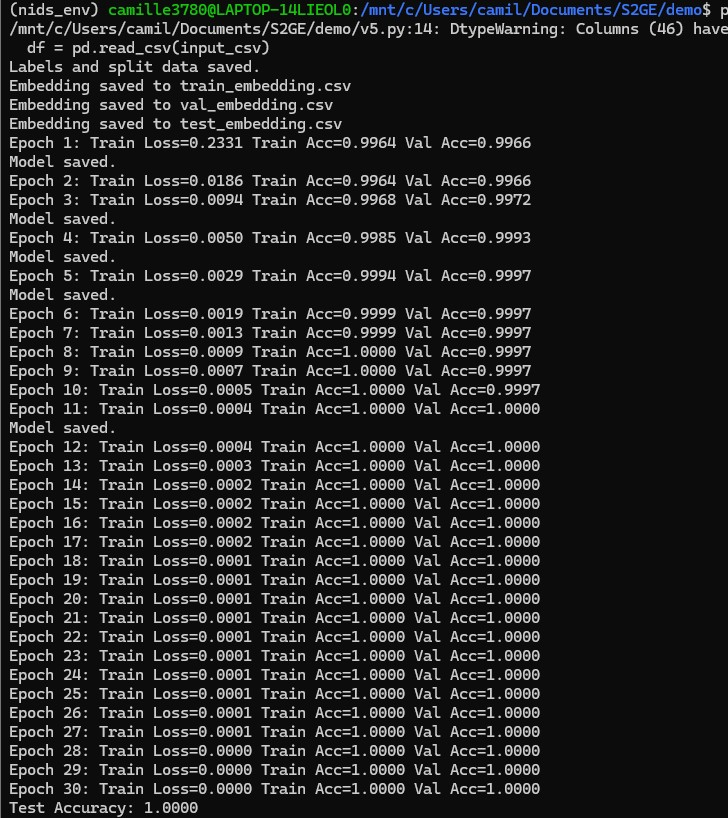
\includegraphics[width = 0.6\textwidth]{image/V8.jpg}
        \caption{Mahalanobis Distances of Result}
        \label{fig:mh_rs}
    \end{figure*}





    \subsubsection{Determine the Anomaly Score}
    After obtaining the semantic vector \(\mathbf{z}\) of each input data point through the MLP encoder, and computing the center point \(\mathbf{c}\) based on all normal training samples, the system evaluates how far each sample deviates from the normal data distribution using the Mahalanobis distance metric.

    The Mahalanobis distance score \(D_M(\mathbf{z})\), quantifies the distance between a sample's semantic representation \(\mathbf{z}\) and the center vector \(\mathbf{c}\), while accounting for the variance and covariance of the embedding space. This distance serves as the anomaly score for each sample.

    To determine whether a sample is anomalous, a threshold \(\tau\) is defined based on the distribution of distances observed in the training data. A sample is classified as anomalous if its Mahalanobis distance exceeds this threshold:

    \begin{equation}
        \text{Anomaly}(z) =
        \begin{cases}
            1 & \text{if } D_M(z) > \tau \\
            0 & \text{otherwise}
        \end{cases}
    \end{equation}

    This threshold-based mechanism enables the system to make binary decisions (normal vs. anomalous) while preserving the interpretability and statistical grounding of the anomaly scores.

    \begin{figure*}[htbp]
        \centering
        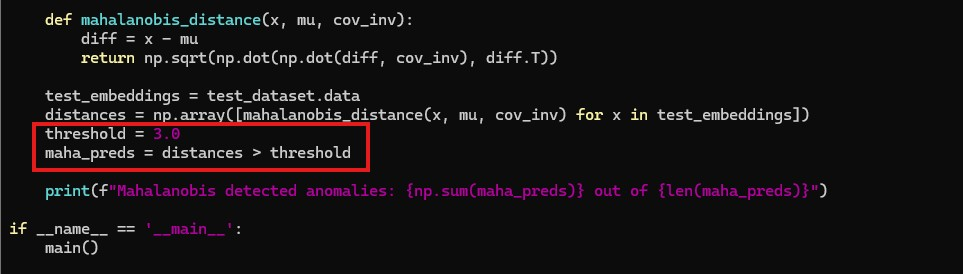
\includegraphics[width = 0.8\textwidth]{image/AnomalyScore.jpg}
        \caption{Calculate and filter the Mahalanobis anomaly score}
        \label{fig:abc}
    \end{figure*}


    Figure~\ref{fig:abc} shows the compute of anomaly score for each data sample, we utilize the Mahalanobis distance to quantify how far each sample deviates from the distribution center of normal data in the latent feature space~\cite{kamoi2020mahalanobis}. The process is as follows:

    \begin{enumerate}
        \item \textbf{Covariance Matrix Estimation:} The empirical covariance matrix is calculated from all latent semantic vectors using the \texttt{EmpiricalCovariance} function, serving as the statistical basis for Mahalanobis distance computation.

        \item \textbf{Definition of Mahalanobis Distance Function:} For each sample vector $\mathbf{x}$, its distance is computed by invoking the \texttt{cov.mahalanobis([x])} method.

        \item \textbf{Anomaly Score Calculation:} The Mahalanobis distance is calculated sequentially for all samples, producing a list of anomaly scores.

        \item \textbf{Anomaly Threshold Setting:} Multiple percentile thresholds (95\%, 96\%, 97\%, 98\%, 99\%) are determined based on the distribution of anomaly scores in the training data to distinguish between normal and anomalous samples.

        \item \textbf{Statistical Output of Anomaly Scores:} The range, mean, and standard deviation of anomaly scores are reported, along with the top anomaly scores from the samples.

        \item \textbf{Anomaly Sample Identification:} Samples exceeding the 99\% percentile threshold are flagged as anomalies, facilitating further evaluation and analysis.
    \end{enumerate}




    \section{Flow} %Chapter 3.2
    This section presents the flow of proposed system. The complete workflow consists of three main components: the preprocessing module, the embedding module, and the Mahalanobis distance module.

    \subsection{Preprocess Module}
    As shown in Figure~\ref{fig:FlowChart}, the system receives the uploaded network packet data and verifies whether its format conforms to the Comma-Separated Values(CSV) format. If the data is not in CSV format, the system will drop the package. In the next stage, the system cleans the data fields, including removing any missing or empty fields from the packets.

    In this experiment we use Pandas and NumPy to data selection and cleaning stage. This includes standardizing column names, removing missing or undefined values, and deleting columns that contain only zeros to reduce noise.

    \begin{figure*}[htbp]
        \centering
        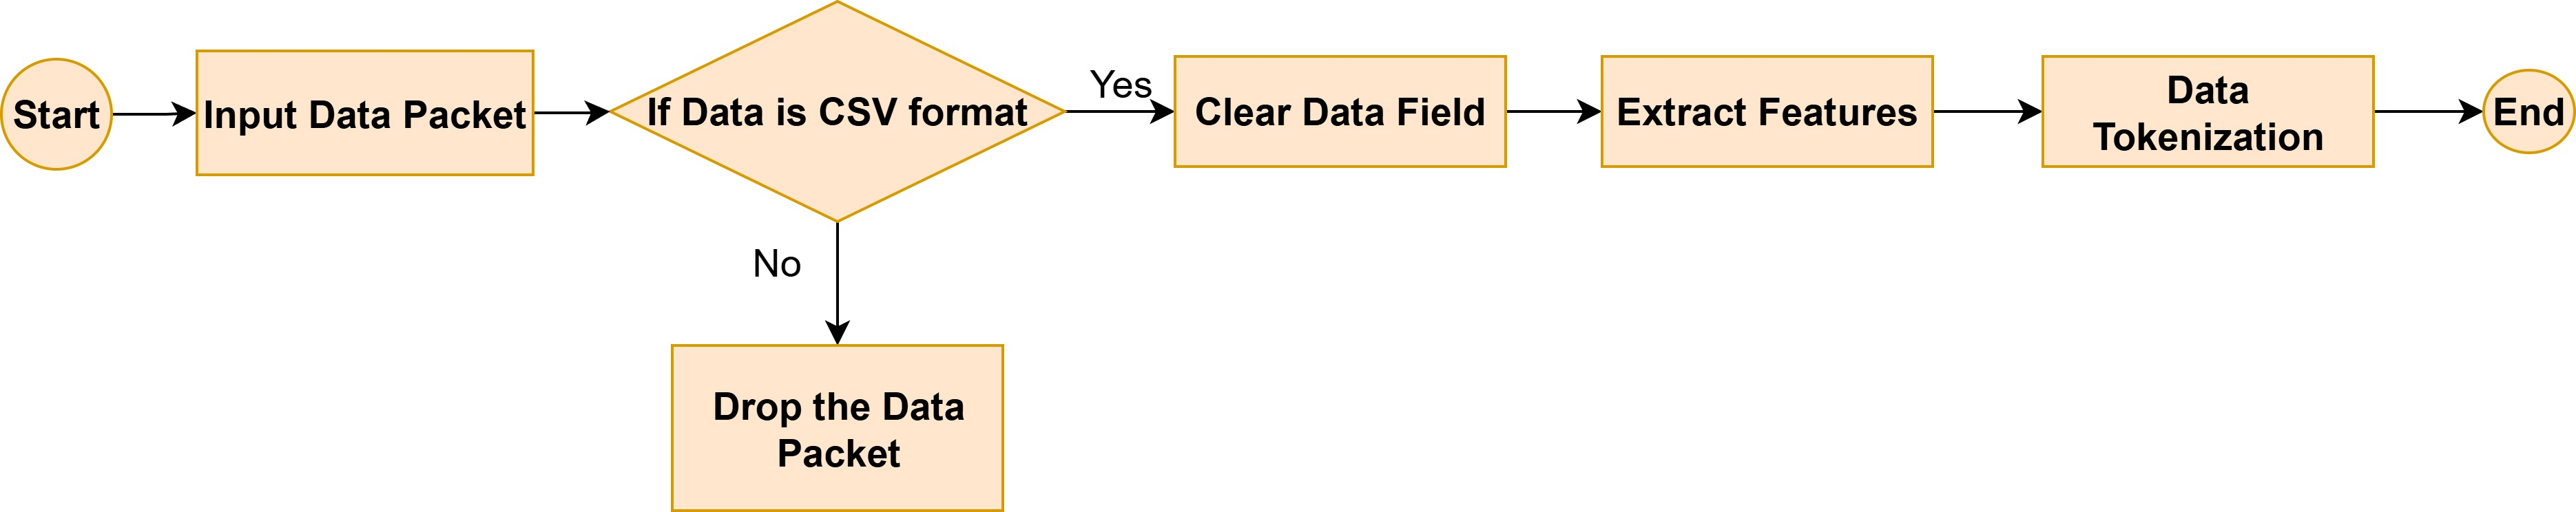
\includegraphics[width = 1\textwidth]{image/FlowChart.jpg}
        \caption{Overview of the Preprocessing Procedure}
        \label{fig:FlowChart}
    \end{figure*}

    We use specific fields related to common anomaly detection features are extracted, such as \texttt{Destination Port}, \texttt{Protocol Type}, and \texttt{Source IP} (\texttt{SrcIP}). These fields serve as important inputs for subsequent module analysis.

    Then, the field names and their respective values are combined into tokens—for example, \texttt{Protocol\:TCP} or \texttt{Port\:80} and fed into a semantic embedding module to be transformed into vectors for further processing.




    \subsection{Embedding Module}
    In Figure~\ref{fig:HashEmbeddingDetail}, this module is responsible for converting the structured semantic token sequence into a vector representation. This module includes Hash Embedding, Flatten to One Class Vector, and MLP to Vector. Each of them contributes to the lightweight and scalable nature of the system. The overall procedure is detailed as follows:

    \begin{figure*}[htbp]
        \centering
        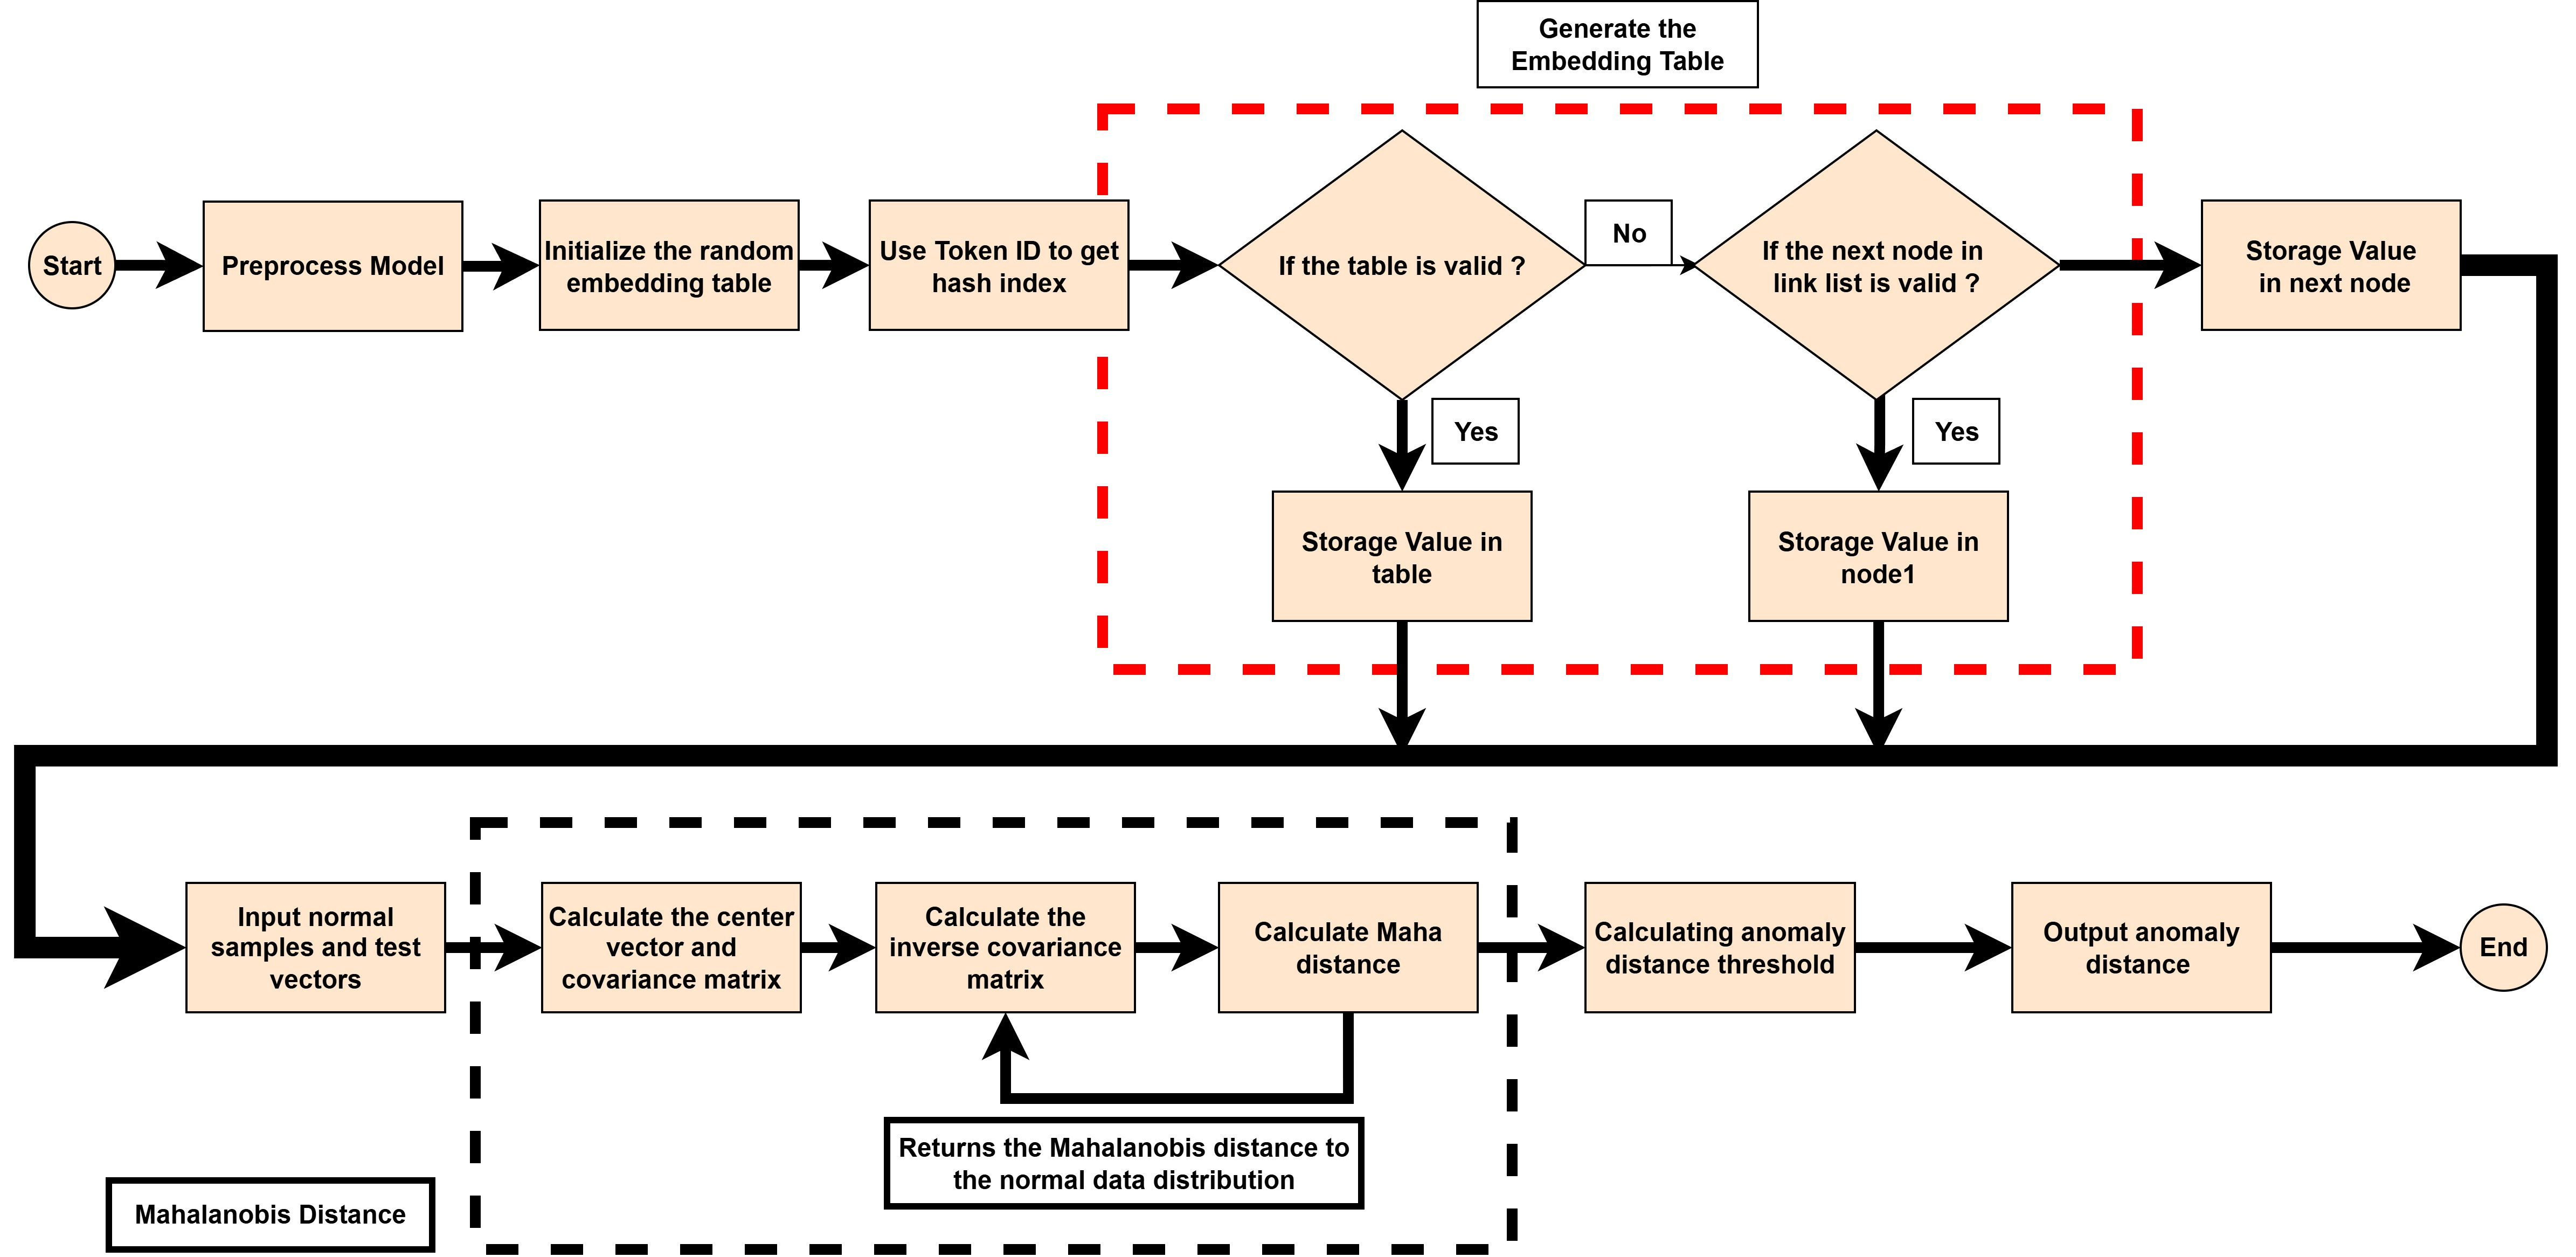
\includegraphics[width = 1\textwidth]{image/embedding.jpg}
        \caption{Overview of the Embedding Procedure Module}
        \label{fig:HashEmbeddingDetail}
    \end{figure*}

    Initially, we use relevant the preprocessing module converts into token IDs. These token IDs are then processed by a non-cryptographic hash function, such as MurmurHash3, which generates hash values. To constrain the hash values within the bounds of the embedding table size to 223, a modulo operation is performed, resulting in a unique embedding table index.

    Upon obtaining the index, the embedding table is queried to retrieve the corresponding embedding vector for the node. Due to the inevitability of hash collisions where distinct tokens may map to the same index—the embedding table employs a linked list structure to store multiple vectors at the same index.





    Formally, for a given token $t = \texttt{Field:Value}$, we compute:

    \begin{equation}
        \text{row\_idx} = \text{MurmurHash3}(\texttt{Field}) \bmod P
    \end{equation}

    \begin{equation}
        \text{col\_idx} = \text{MurmurHash3}(\texttt{Value}) \bmod P
    \end{equation}

    where $P = 223$ is a small prime number chosen to reduce the probability of hash collisions and to ensure efficient modular indexing.

    The resulting $(\text{row\_idx}, \text{col\_idx})$ pair identifies a unique coordinate in the 2D embedding table $\mathbf{E} \in \mathbb{R}^{P \times P \times d}$, where each entry holds a trainable $d$-dimensional embedding vector.




    \subsection{Mahalanobis Distance Module}
    In this section, we introduce an anomaly detection approach that leverages the Mahalanobis distance as the fundamental metric for decision making. We begin by comparing each data vector to a defined center point, followed by calculating the corresponding loss to measure deviation. Finally, this loss is used to determine the anomaly score that indicates the likelihood of abnormality.

    Given $N$ semantic vectors $\mathbf{z}_1, \dots, \mathbf{z}_N$ generated from benign training data, we first compute the statistical mean (center) vector $\boldsymbol{c}$ and covariance matrix $\boldsymbol{\Sigma}$:

    \begin{equation}
        \boldsymbol{c} = \frac{1}{N} \sum_{i=1}^{N} \mathbf{z}_i
    \end{equation}

    \begin{equation}
        \boldsymbol{\Sigma} = \frac{1}{N - 1} \sum_{i=1}^{N} (\mathbf{z}_i - \boldsymbol{c})(\mathbf{z}_i - \boldsymbol{c})^T
    \end{equation}



    For any test vector $\mathbf{z}$, the Mahalanobis distance $D_M(\mathbf{z})$ with respect to the normal distribution is calculated as defined in Equation~(\ref{eq:mahalanobiseq}).




    A larger distance indicates a greater deviation from the normal behavior, suggesting a higher probability of being anomalous.



    \begin{figure*}[htbp]
        \centering
        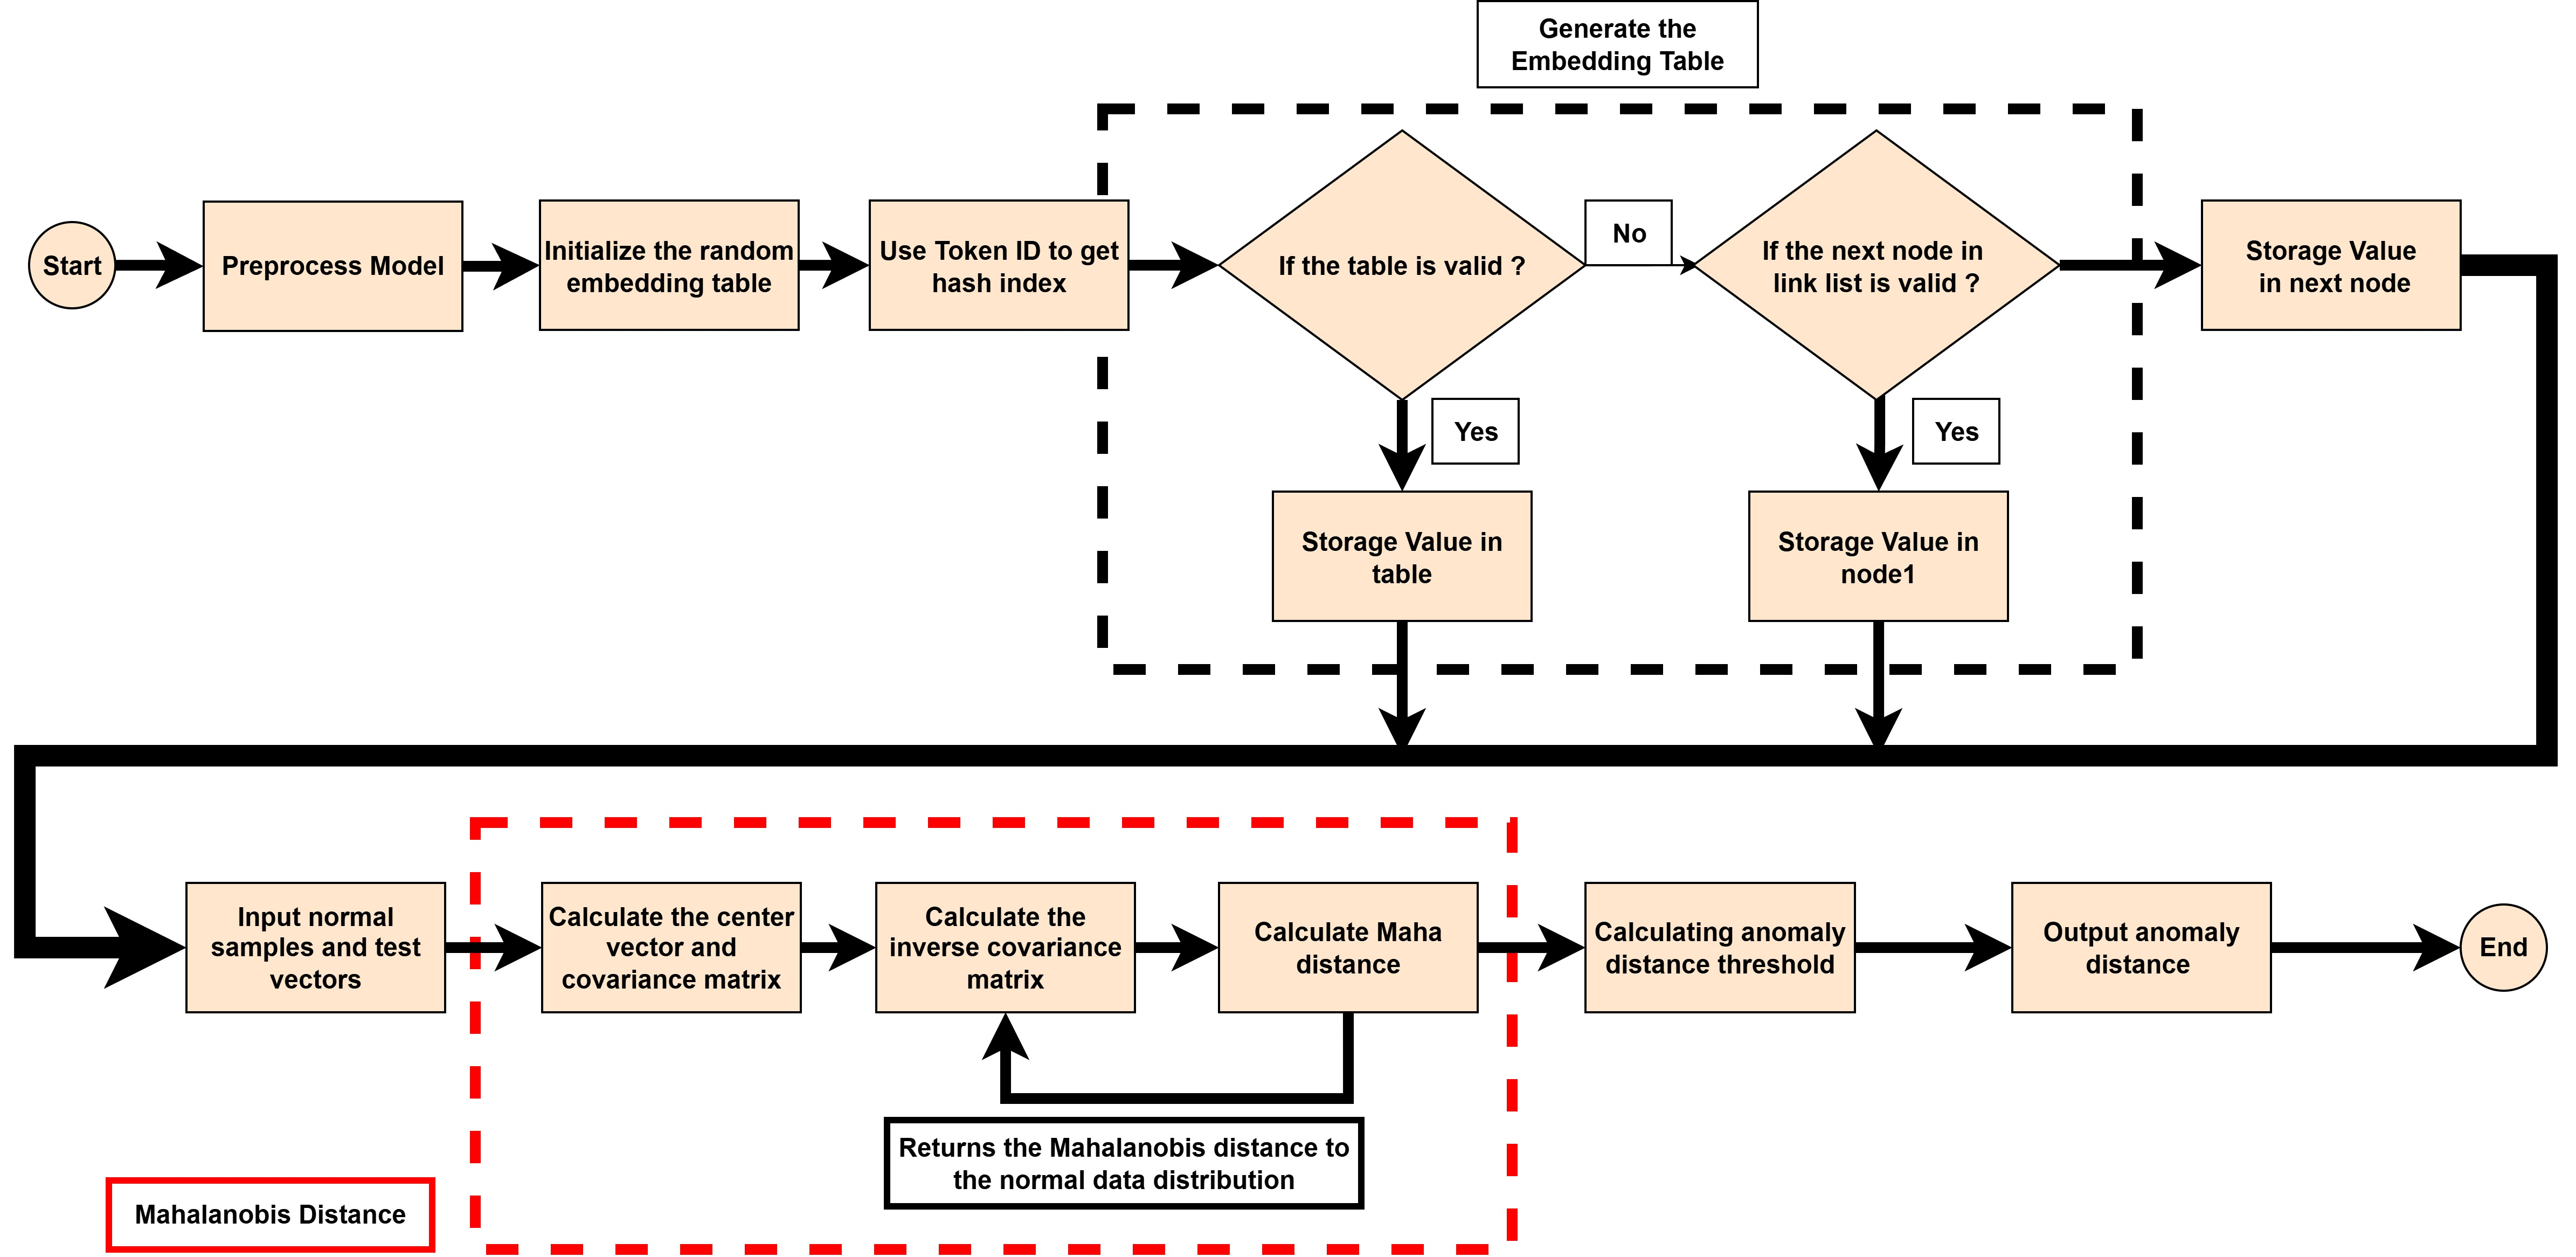
\includegraphics[width = 1\textwidth]{image/MD.jpg}
        \caption{Mahalanobis Distance Anomaly Detection Process}
        \label{fig:EmbeddingFlow}
    \end{figure*}


    \newpage
    We define a threshold $\tau$ based on the distribution of $D_M(\cdot)$ in the training data (e.g., 95th percentile).


    Anomaly detection process begins with the input of normal training samples alongside the test vectors requiring evaluation. From the normal samples, the center vector (mean vector) and the covariance matrix are computed to characterize the distribution of the normal data. Subsequently, the inverse of the covariance matrix is calculated to facilitate the computation of the Mahalanobis distance for each test vector. The Mahalanobis distance measures how far a given test sample deviates from the normal data distribution, accounting for the data's covariance structure. All computed distances serve as anomaly scores representing the degree of deviation. These scores are stored in an array for systematic processing. Statistical measures, including the mean and standard deviation of the anomaly scores, are then derived to establish a threshold. Samples whose anomaly scores exceed this threshold are classified as anomalous, enabling effective discrimination between normal and abnormal instances.



    \begin{equation}
        \text{Anomaly}(\mathbf{z}) =
        \begin{cases}
            1, & \text{if } D_M(\mathbf{z}) > \tau \\
            0, & \text{otherwise}
        \end{cases}
    \end{equation}

    This distance reflects the statistical deviation of a sample from the center of the normal data distribution in the multi-dimensional feature space, taking into account the correlations among different features. When the Mahalanobis distance $MD(\mathbf{z})$ exceeds a predetermined anomaly threshold $\tau$, the sample is classified as anomalous; otherwise, it is considered normal. The threshold can be adjusted based on the statistical characteristics of the distance distribution in the training data (e.g., set as the mean plus three times the standard deviation) to balance the sensitivity and false alarm rate of the anomaly detection. Through this approach, the system can effectively identify anomalous events that deviate significantly from the normal distribution, thereby improving the accuracy and robustness of anomaly detection.


    \begin{itemize}
        \item \textbf{Input}: Semantic vector $\mathbf{z} \in \mathbb{R}^k$ (from MLP)
        \item \textbf{Output}: Anomaly score $D_M(\mathbf{z})$ and binary decision
        \item \textbf{Computation}: Based on $\boldsymbol{c}$ and $\boldsymbol{\Sigma}$ estimated from training data
    \end{itemize}



    \begin{itemize}
        \item \textbf{Unsupervised}: Requires only benign data for training
        \item \textbf{Interpretable}: Outputs a clear statistical distance as anomaly score
        \item \textbf{Statistically Sound}: Incorporates feature correlation via covariance
        \item \textbf{Efficient}: Only requires mean and covariance estimation once during training
    \end{itemize}




\end{ZhChapter}